%!TEX root = ../hutbthesis_main.tex
\chapter{绪论}

\section{研究背景与意义}

在一次航班离港流程中，飞机从停机位推出到进入滑行路线，看起来只是周转链条中的一个短环节，但它实际上同时牵涉机坪交通、廊桥区域安全、地勤人员协同和后续放行节奏。牵引车需要在飞机前起落架附近低速靠近，车身周围又存在机翼、发动机、廊桥、保障车辆和地面标线等多种约束。任何一次偏航过大、停车不及时或目标识别错误，都可能使简单的推出作业演变为安全事件。因此，飞机牵引与推出并不是单纯的``车辆驾驶''问题，而是一个典型的低速、高精度、多约束协同作业问题\cite{ref1,ref2}。

目前多数机场的推出与牵引仍以人工驾驶牵引车、机务或指挥员目视协同为主。该方式在经验丰富、交通密度较低的情况下较为可靠，但其稳定性很大程度取决于人员状态和现场沟通质量。航班高峰、夜航、雨雾天气以及机坪车辆交叉运行时，人工判断容易受到视距、噪声和遮挡影响，牵引路径规划、翼尖安全距离判断、前起落架对准等环节都可能出现误差。对智慧机场而言，这类高度依赖人工经验的作业环节，会限制地面运行系统继续向闭环调度和自动执行方向发展。

相关资料表明，机场地面运行阶段的安全风险并不低，推出、牵引和低速滑行是典型的风险集中环节之一，常见问题包括牵引车与机体接触、翼尖剐蹭、人员误入作业区域等。同时，地面运行延误还会沿航班计划向后传递，使单个机位或单个航班的问题进一步影响后续起飞排序和机坪资源利用。因此，提高牵引作业的自动化水平，不仅有助于降低局部操作风险，也有助于提升机场地面运行的整体稳定性\cite{ref3,ref4,ref5,ref6}。

从技术发展看，机场场面运行系统正由传统SMGCS向A-SMGCS（Advanced Surface
Movement Guidance and Control
System）升级。A-SMGCS强调对地面目标的监视、引导、冲突预警和运行协同，为机场车辆与航空器的统一管理提供了系统框架\cite{ref2,ref3,ref4}。不过，现有研究和工程应用更多集中在飞机滑行监视、场面交通管理和冲突告警层面，对``牵引车---飞机''这一强耦合、近距离、低速精对准对象的自动控制研究仍不充分。尤其是在牵引车接近前起落架、姿态对齐、低速停车和后续推出这一连续过程中，仍缺少面向仿真验证的完整方法。

基于上述背景，本文选择以高保真仿真环境为研究支撑，围绕机场牵引车与飞行器的协同控制展开建模、感知、路径规划和控制验证。通过在ROS与Gazebo环境中构建牵引车、飞机目标和机坪作业场景，可以在较低成本下复现实车试验中难以频繁开展的对接过程，观察车辆转向、速度、目标识别和安全约束之间的相互影响\cite{ref11,ref12,ref13}。这对于后续自动牵引系统的样机设计、控制算法调试以及机场地面作业智能化研究都具有现实意义。

\section{国内外研究现状}

\subsection{机场牵引与地面自动化研究现状}

机场地面自动化研究的出发点，是在不降低安全裕度的前提下减少人工重复操作，并提高机坪资源的利用效率\cite{ref1,ref2,ref3,ref4}。飞机推出与牵引处在航班周转和场面交通之间：一方面，它需要服从停机位、滑行通道、速度限制和指挥流程等机场运行规则；另一方面，它又要求牵引车在飞机前起落架附近完成低速对准、连接和稳定牵引。因此，该环节既有车辆控制问题，也有机场运行组织问题。

国外较早围绕``无发动机滑行''和自动牵引开展研究。以TaxiBot、e-Taxi等方案为代表，相关工作尝试通过牵引车或机轮电驱系统减少飞机发动机地面运行时间，从而降低燃油消耗、噪声和排放\cite{ref6,ref8,ref9}。Zaninotto等面向自动牵引作业提出调度与路径规划方法，通过冲突检测和时序优化减少牵引车之间、牵引车与飞机之间的运行冲突，说明自动牵引在提高滑行效率和减少人为差错方面具有可行性\cite{ref7}。此外，也有研究从牵引车---飞机组合体的制动、转向和纵向耦合特性入手，为低速牵引控制提供动力学基础\cite{ref6,ref10,ref19}。

在机场系统层面，SESAR等项目持续推动场面运行从单点自动化向系统协同自动化发展。A-SMGCS的相关研究强调将监视、路径引导、冲突预警与运行管理结合起来，使机场能够对航空器和车辆目标进行更精细的状态管理\cite{ref2,ref3,ref4}。这类研究为自动牵引提供了上层运行框架，但其重点通常不在牵引车末端对接控制本身，而在于更大范围的场面交通监视与运行调度。

国内关于飞机牵引滑行和地面运行智能化的研究起步相对较晚，但近年来进展明显。孙艳坤等对飞机牵引滑行技术进行了系统综述，内容涉及牵引装备类型、动力学特性、运行模式和发展趋势，并指出自动牵引与智能调度是后续重要方向\cite{ref6}。在规范层面，中国民航局发布的A-SMGCS相关技术指南和行业标准，也为机场场面运行的信息化和智能化建设提供了依据\cite{ref1,ref2}。不过，从现有公开研究看，国内工作仍较多停留在系统规划、装备综述或单一算法分析层面，对牵引车自动接近飞机、对准前起落架并完成安全停车这一末端过程的仿真验证仍然不足。

因此，本文的研究切入点并不是重新讨论机场自动化的宏观框架，而是将问题压缩到一个更具体的作业单元：在给定机场作业规则和车辆结构约束下，牵引车如何识别飞机目标、生成可执行路径，并以稳定方式完成对接。这个问题更贴近实际工程调试，也更适合通过ROS-Gazebo联合仿真进行反复验证。

\subsection{协同控制与路径规划方法研究现状}

从方法上看，机场牵引自动化可归入移动机器人导航和智能车辆控制范畴，但它又不能完全照搬普通道路自动驾驶或仓储AGV的方案\cite{ref17,ref18,ref19,ref20,ref28}。原因在于，牵引车面对的是航空器这一高价值目标，运行区域空间狭窄、规则刚性强，而且最终对接阶段对横向误差和姿态误差都十分敏感。也就是说，路径规划不仅要``走得到''，还要``转得过、停得住、对得准''。

图搜索与采样类算法是路径规划研究中的基础方法。A*、Dijkstra等图搜索算法结构清晰、结果可解释性强，适合在机场滑行道、机坪通道等规则环境中生成全局参考路径\cite{ref22,ref23}；RRT及其改进算法则更适合在连续空间中快速搜索可行路径，常用于机器人和自动车辆的运动规划\cite{ref20,ref21,ref24}。这类方法的优势在于稳定和易于检查，但在动态障碍较多、局部空间受限或车辆曲率约束较强时，单独使用往往需要额外的平滑、重规划和可行性筛选。

智能优化算法也被广泛用于路径规划问题。例如蚁群算法、粒子群算法等可以把路径长度、安全距离、能耗或时间代价写入统一目标函数，对多约束规划具有一定灵活性。但这类算法通常对参数设置较敏感，收敛速度和解的稳定性会随场景复杂度变化而波动。机场牵引属于安全敏感任务，若规划结果难以解释或每次计算结果差异较大，工程应用就会受到限制。

近年来，强化学习和深度强化学习在复杂动态环境决策中受到关注。它们能够通过与环境交互学习策略，对未知障碍或非结构化场景具有一定适应能力。但机场场景对安全性、可验证性和监管合规性要求较高，单纯依赖黑箱策略并不合适；同时，强化学习对训练数据规模和仿真真实性依赖较强，若仿真与真实机坪差异较大，策略迁移效果也难以保证。

综合来看，适合本课题的路线应是分层式、融合式的。上层规划尽量保留机场规则、车辆曲率和安全距离等显式约束，保证路径可解释、可检查；下层控制根据实时感知误差进行局部修正，解决对接过程中的小偏差和动态干扰。这样的框架既不过分依赖单一智能算法，也能避免纯规则方法在复杂局部场景中反应不足的问题，为后续牵引车---飞机协同控制提供了更稳妥的技术基础\cite{ref25,ref28}。

\section{研究内容与技术路线}

本文以机场飞机推出与牵引作业为应用背景，重点研究牵引车与飞行器在低速近距场景下的协同控制问题。课题并不追求单一算法指标，而是围绕``建模---感知---规划---控制---仿真验证''这条链路展开：先把机场牵引作业抽象成可计算的问题，再利用仿真平台检验车辆能否按预期完成目标识别、接近、对准和停车。结合本文已经开展的ROS/Gazebo建模、SolidWorks车辆模型导入、双桥转向控制调试等工作，主要研究内容和技术路线如图~\ref{fig:1-1} 所示，具体内容如下。

\begin{enumerate}[label=（\arabic*）,leftmargin=2em]
\item \textbf{机场牵引作业流程建模与问题抽象}。从停机位推出和前起落架对接过程出发，分析牵引车、飞机、机坪通道、禁行区域和障碍物之间的关系。根据作业顺序，将自动牵引过程划分为目标确认、初始接近、姿态对准、微动对接和停车保持等阶段，并把实际约束转化为状态变量、控制输入和安全边界。该部分的目的，是为后续控制算法提供一个统一的问题描述，而不是只停留在场景文字说明上。
\item \textbf{面向自动对接的飞机辅助感知方法}。在仿真环境中，飞机前起落架区域被设计为主要识别对象，通过设置可识别标识，使牵引车能够获取目标身份、相对距离、横向偏差和姿态偏差等信息。视觉传感器用于目标确认与相对位姿估计，激光雷达、超声波或等效近距传感器用于安全距离判断。该部分重点解决``牵引车如何知道自己应该接近哪一架飞机、朝哪个方向对准、何时需要停车''的问题。
\item \textbf{多约束条件下的路径规划与协同控制方法}。在车辆运动学模型和感知误差接口的基础上，设计自动接近与对接控制方法。全局层面，根据机场运行规则和车辆曲率约束生成可执行参考路径；局部层面，根据实时感知误差对速度和转向进行在线修正。控制策略需要同时考虑低速稳定性、转向角限制、安全距离、终端停车阈值和对接姿态要求。本文采用分层控制思路，将模式管理、局部规划、误差反馈和执行器映射分开处理，使算法结构更便于在ROS节点中实现。
\item \textbf{基于高保真模拟器的系统集成与验证}。依托ROS与Gazebo搭建牵引车---飞机对接仿真系统。车辆模型由SolidWorks建立并经URDF/STL等形式导入Gazebo，前后桥转向关节和四个驱动车轮通过控制器实现位置和速度控制，传感器模型挂载于车体前部。通过设置典型机场作业场景，对牵引车模型加载、转向回中、轮速控制、目标接近和停车判定等功能进行验证，并从安全性、路径平滑性和控制稳定性等角度分析系统表现。
\item \textbf{牵引车辆结构与动力系统的工程化思考}。在完成仿真和控制算法研究的同时，结合机场牵引车实际需求，对车辆结构、动力布置和维护便利性进行初步分析。该部分不作为完整机械设计展开，而是从工程实现角度讨论车辆硬件结构与控制策略之间的关系，例如双桥转向结构对小半径机动和精细对位的影响、动力响应对低速控制稳定性的影响等，为后续实物样机或半实物平台研究提供参考。
\end{enumerate}

\begin{figure}[htbp]
    \centering
    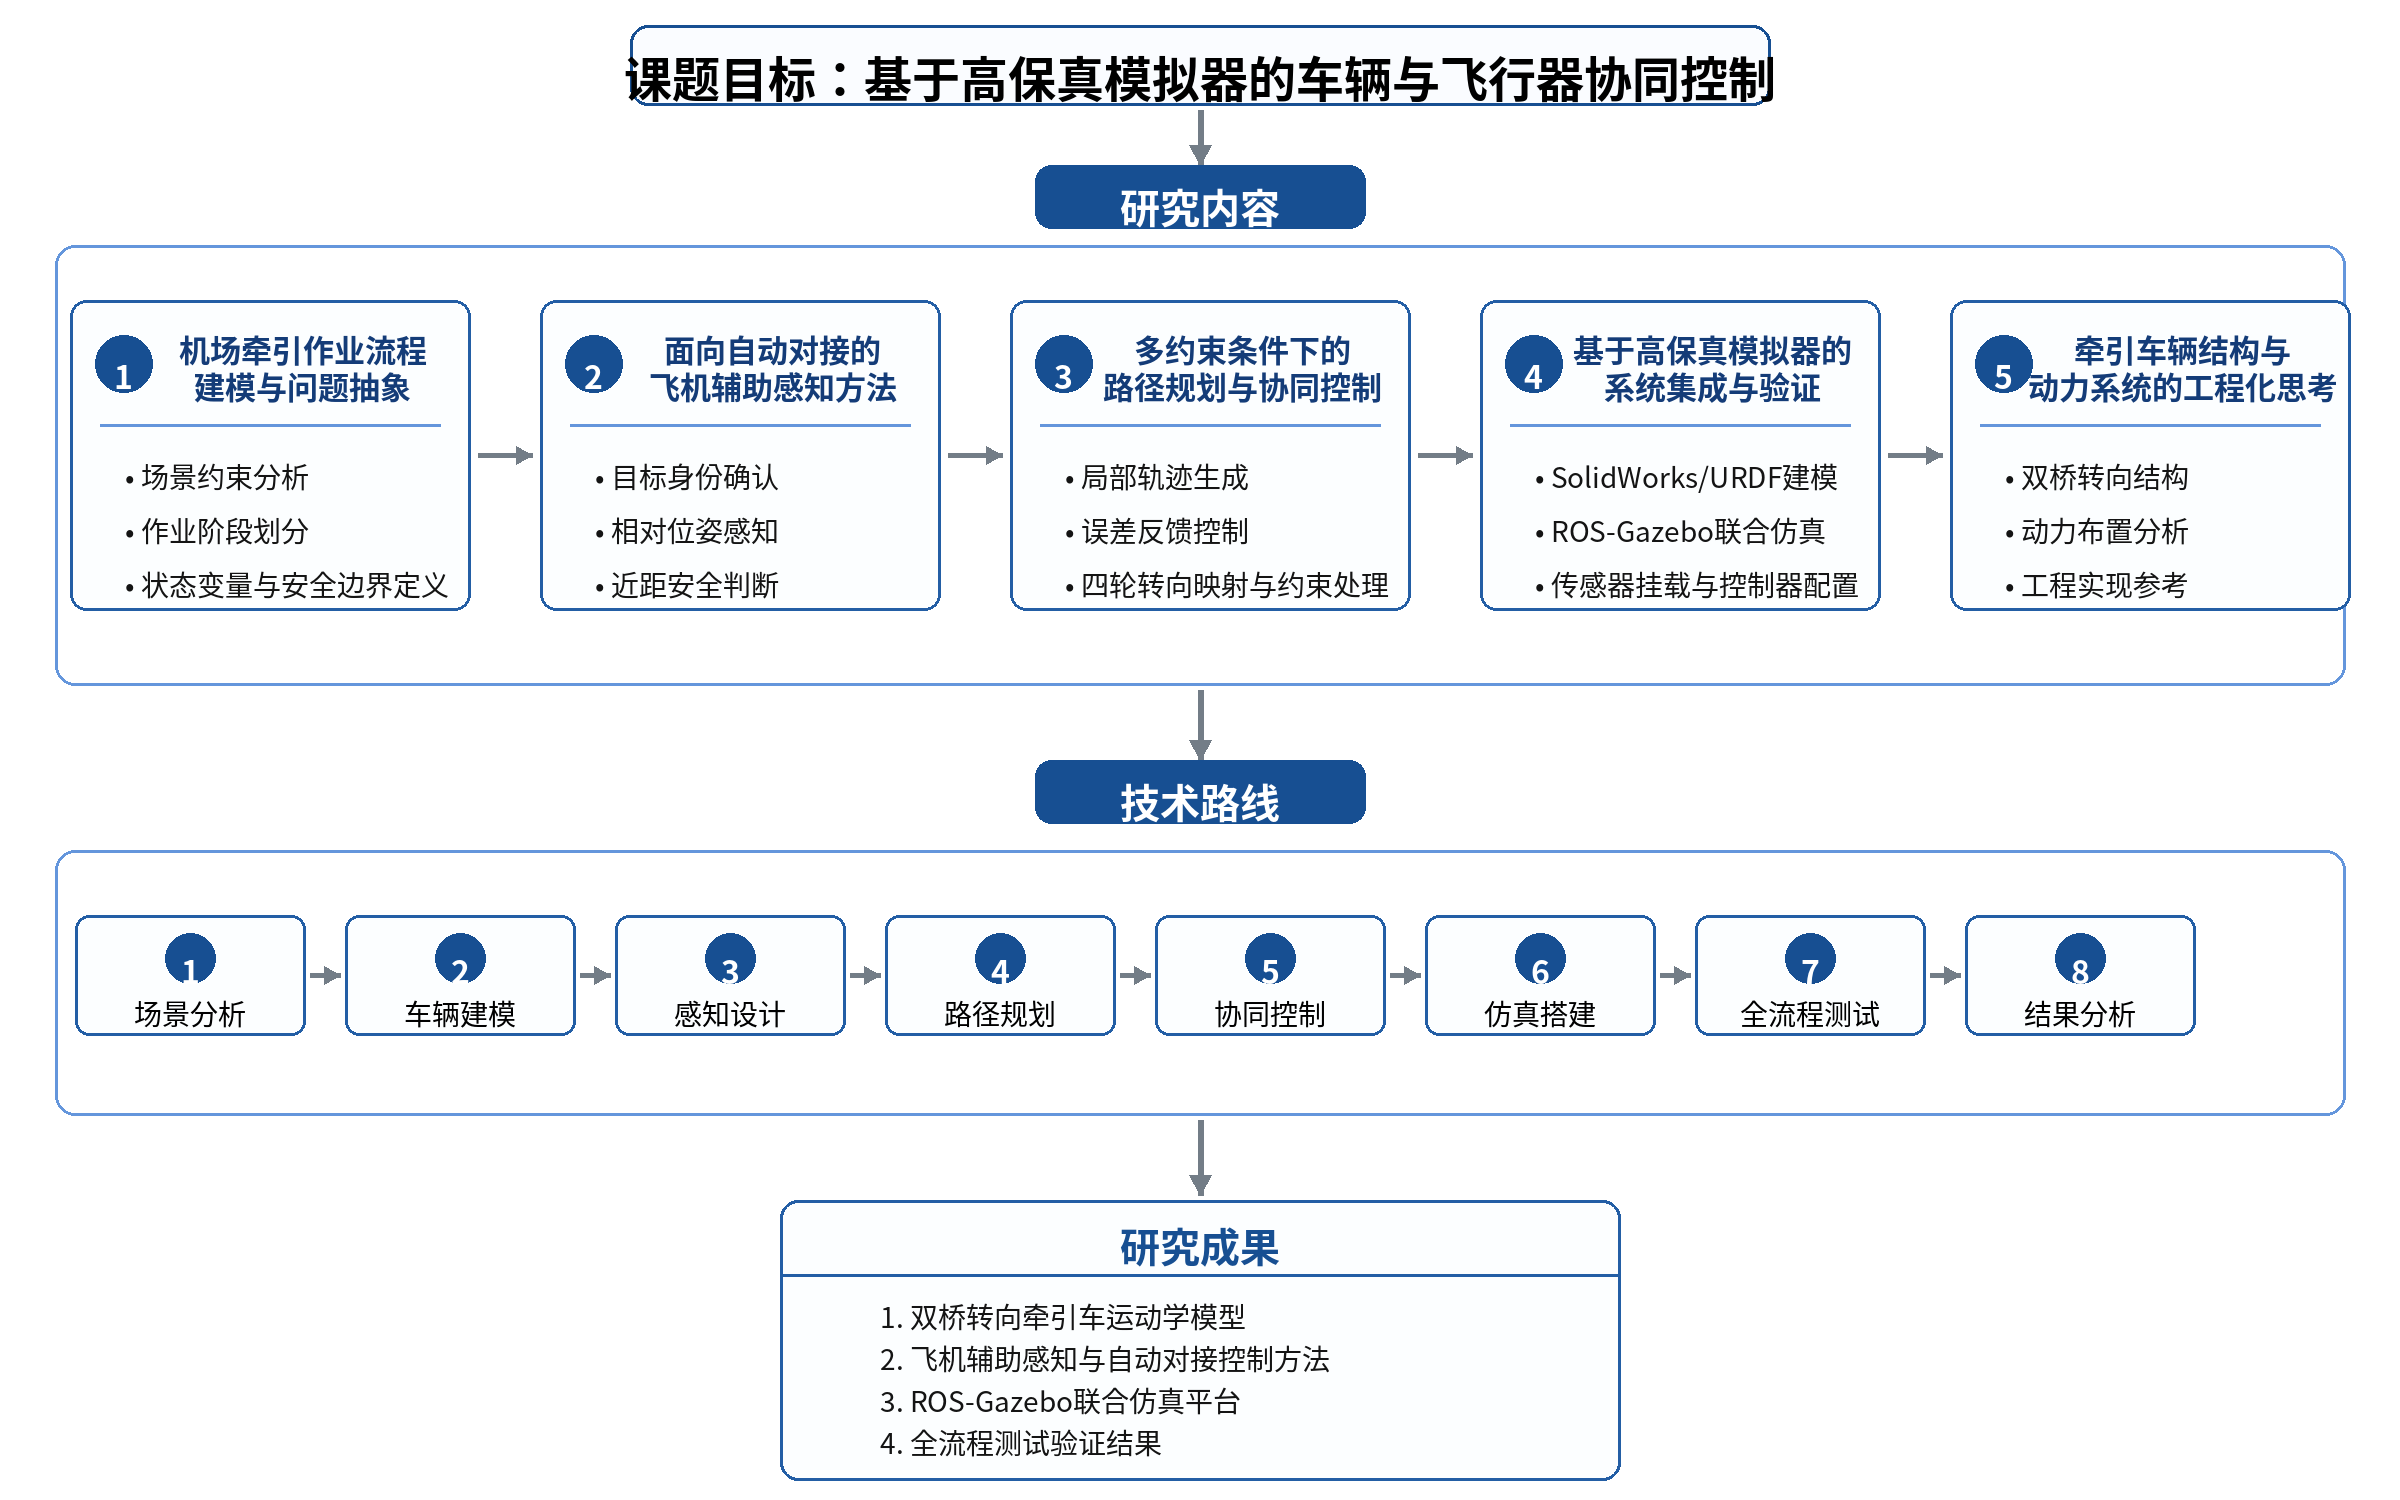
\includegraphics[width=5.76806in,height=3.76181in]{figures/image2.png}
    \caption{研究内容与技术路线图}
    \label{fig:1-1}
\end{figure}
